\documentclass[10pt, fleqn, twocolumn]{jsarticle}
\usepackage[dvipdfmx]{graphicx,color}
\usepackage{amsmath}
\usepackage{here}
\usepackage[top=20truemm,bottom=20truemm,left=15truemm,right=15truemm]{geometry}
\usepackage{fancyhdr}
\usepackage{multirow}
\usepackage{nidanfloat}
\usepackage{subcaption}
\usepackage{titlesec}
\usepackage{tabularx}
\captionsetup{labelsep=space}

% % セクションの設定
\titleformat*{\section}{\normalsize\bfseries}

% % 章・節・項番号のフォントの変更
\renewcommand{\headfont}{\bfseries}

% 図表番号の設定
\renewcommand{\figurename}{Fig.~}
\renewcommand{\tablename}{Tab.~}

%ヘッダーの設定
\pagestyle{fancy}
\lhead{修士論文中間発表会}
\rhead{2023年8月9日}
%ヘッダーの罫線を無くす
\renewcommand{\headrulewidth}{0pt}

\begin{document}
%一段組にして, タイトル, 所属, 氏名を記載
\twocolumn[
\begin{center}
  \large{
    CNNに基づく気液二相噴流のパッシブ音響識別に関する研究\\
    (ノイズ耐性の評価とGrad-CAMによる視覚的説明)
  }
\end{center}
\begin{flushright}
  機械工学専攻 マイクロ熱工学領域 芝原研究室 三上奈生
\end{flushright}
~
]

\section{緒言}
気液二相流の流動状態は熱・物質輸送と強く関係し, 構造物の疲労・腐食などの潜在的な問題を引き起こす場合もある~\cite{Yao2019}.
例えば, ナトリウム冷却高速炉(SFR)では蒸気発生器(SG)内の伝熱管に貫通き裂が生じると, 水/蒸気がナトリウム中にリークし, 気液二相噴流による伝熱管の損耗(ウェステージ)が生じる恐れがある.
ウェステージ現象は水リーク率によって大別され, 微小の水リーク率では管壁の自己損耗(セルフウェステージ)や高温化による強度低下が生じ, 水リーク率が増大すると隣接する伝熱管の二次的な破損が生じる.
そのため, 気液二相噴流の流動状態を高速かつ高精度で検知・識別する手法の開発が求められている.

この識別手法として, 本研究では畳み込みニューラルネットワーク(CNN)とパッシブ音響法に着目する.
音響法は応答性に優れており, SG内部のような不可視領域にも適用可能である.
また, CNNは既存手法~\cite{Mikami2023a}よりもノイズ耐性に優れており, 実機のような高レベルノイズ環境での識別にも対応できる可能性がある.
さらに, 近年AIには説明責任が求められており, CNNに対する入力と予測に対して局所的な説明を与える勾配加重クラス活性化マッピング(Grad-CAM)~\cite{Selvaraju2017}の導入が進んでいる.
しかし, ノイズ環境下で気液二相噴流の音響識別を行った例やGrad-CAMを応用した例は少ない.
以上を踏まえ, 本研究ではCNNに基づく気液二相噴流のパッシブ音響識別手法のノイズ耐性の評価, およびGrad-CAMによる予測根拠の可視化を行う.

\begin{table*}[b]
  \centering
  \caption{Accuracy of ResNet18 with best TFRs for ${\rm SNR}=0,-4,-8,-12,-16,{\rm and}-20$ dB.}
  \label{tab:accuracy_of_resnet18}
  \begin{tabularx}{\textwidth}{X|XXXXXX}
    \hline
    SNR & 0 dB & $-4$ dB & $-8$ dB & $-12$ dB & $-16$ dB & $-20$ dB \\
    \hline
    Best TFR & STFT & STFT & STFT & STFT & SWT & SWT \\
    Accuracy & $98.80\pm1.63$\% & $97.50\pm2.66$\% & $94.70\pm4.83\%$ & $92.35\pm5.47$\% & $86.55\pm5.62$\% & $69.15\pm9.11$\% \\
    \hline
  \end{tabularx}
\end{table*}

\section{実験および時間周波数表現の作成}
まず, バックグラウンド音を模擬した水流動音, 異常音を模擬した気液二相噴流音の測定実験を行った.
前者では配管内部の水流動音を60 s間測定し, 後者では孔径0.15, 0.17, 0.20 mmのノズルからの気液二相噴流音をそれぞれ60 s間測定した.
各実験の詳細な条件や音源の物理については筆者らの文献~\cite{Mikami2023a,Mikami2023b}に記載されている.
次に, 得られた音響データに対して, 先行研究~\cite{Zhang2021}と同様に短時間フーリエ変換(STFT), 連続ウェーブレット変換(CWT), シンクロスクイーズドウェーブレット変換(SWT)を用いた時間周波数解析を行い, CNNに入力する時間周波数表現(TFR)を作成した.
各TFRは0.1 sの時間間隔で作成され, $0\sim22.05$ kHzの周波数帯における信号強度分布を表し, CNNに入力される際は縦・横224ピクセル, RGB3チャンネルの画像情報に変換される.
また, ノイズ環境下を再現するために信号対ノイズ比(SNR)を$0, -4, -8, -12, -16, -20$ dBと変化させた場合についてTFRの作成を行った.



\section{CNNおよびGrad-CAMの理論}
本研究では, 大規模画像認識コンテスト(ILSVRC)で優秀な成績を収めたAlexNet, VGG16, ResNet18を分類器として用い, セルフウェステージ現象を想定して水流動音1種(Class W)および気液二相噴流音3種(Class J0.15, Class J0.17, Class J0.20)の計4種の音を分類するようにCNNを構築した.
各SNRにおいて, AlexNet, VGG16, ResNet18のCNN3種とSTFT, CWT, SWTのTFR3種を組み合わせた全9手法の性能評価を行った.

また, CNNの判断根拠を可視化する手法としてGrad-CAMを導入した.
Grad-CAMでは, CNNが予測したクラスが$c$であるときの出力を$y_c$としたとき, 出力$y_c$に対する要素数$Z$の特徴マップ$A^k$の勾配の平均$\alpha_c^k$を次式により求める.
\begin{align}
  \label{eq:neuron_importance_weight}
  \alpha_c^k=\frac{1}{Z}\sum_i\sum_j\frac{\partial{y_c}}{\partial{A_{ij}^k}}
\end{align}
この勾配の平均$\alpha_c^k$が大きいほど, 特徴マップ$A^k$が出力$y_c$により大きな影響を与えたと考えることができる.
そして, 次式のように勾配の平均$\alpha_c^k$と特徴マップ$A^k$の積にReLU関数を施すことで, 出力$y_c$に対する判断根拠をヒートマップとして表すGrad-CAMが得られる.
\begin{align}
  \label{eq:grad-cam}
  L_c^{\textrm{Grad-CAM}}={\rm ReLU}\left(\sum_k\alpha_c^kA^k\right)
\end{align}

\begin{figure}[t]
  \centering
  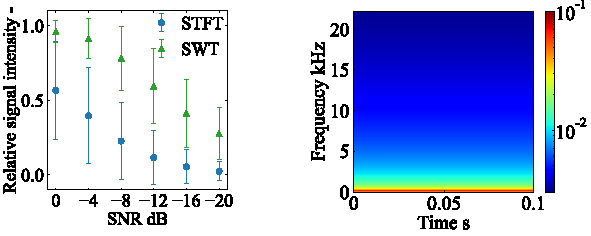
\includegraphics[height=3.5cm]{swt_property.pdf}
  \caption{Left: Maximum relative signal intensity of gas-liquid jet sounds of STFT and SWT; right: intensity distribution of scale parameter terms of SWT.}
  \label{fig:swt_property}
\end{figure}
\begin{figure}
  \centering
  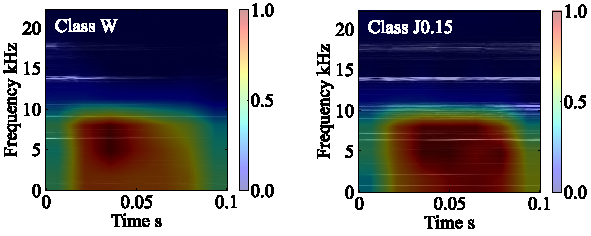
\includegraphics[height=3.5cm]{grad-cam_stft.pdf}
  \caption{Visual explanation of $\rm ResNet18+STFT$ decision for ${\rm SNR}=-12$ dB (left: Class W; right: Class J0.15).}
  \label{fig:grad-cam_snr-12}
\end{figure}
\begin{figure}
  \centering
  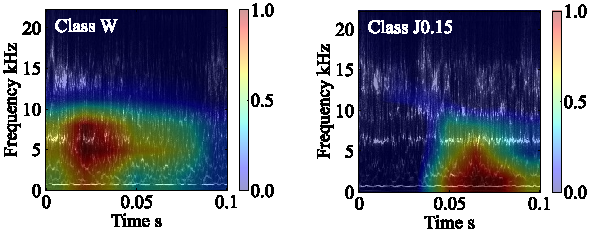
\includegraphics[height=3.5cm]{grad-cam_swt.pdf}
  \caption{Visual explanation of $\rm ResNet18+SWT$ decision for ${\rm SNR}=-20$ dB (left: Class W; right: Class J0.15).}
  \label{fig:grad-cam_snr-20}
\end{figure}

\section{結果と考察}
\subsection{ノイズ耐性の評価}
Tab.~\ref{tab:accuracy_of_resnet18}に全てのSNRで最良手法となったResNet18の精度を示す.
SNRが小さいほどResNet18の精度は低下したが, これはSNRの減少に伴いノイズ強度が増大することを考えると妥当である.
また, ノイズ強度が着目信号強度の100倍となる${\rm SNR}=-20$ dBの高レベルノイズ環境下においても, ResNet18は$69.15\%$の精度を示した.
この結果から, ノイズ環境下での気液二相噴流の識別においてCNNの耐ノイズ性が機能していることが分かる.

また, Tab.~\ref{tab:accuracy_of_resnet18}に示すように${\rm SNR}=0,-4,-8,-12$ dBではSTFTが最高精度に達したTFRとなった.
これは, 元信号の周期性やSTFTがもつ一定の時間・周波数解像度に起因すると考えられる.
一方, ${\rm SNR}=-16,-20$ dBではSWTが最高精度に達したTFRとなった.
これらのSNRでは, 支配的な水流動音に対する気液二相噴流音の信号強度が強く表れていることが重要であると考えられる.
そこで, 気液二相噴流音と水流動音の信号強度の差を気液二相噴流音の相対信号強度と定義し, 気液二相噴流音の特徴周波数帯である約$1500\sim5000$ Hzにおける相対信号強度の最大値を計算した.
その結果がFig.~\ref{fig:swt_property}の左図であり, SWTはSTFTよりも大きな値を示しており, 特に${\rm SNR}=-20$ dBでは約10倍の差となった.
このことから, SWTはSTFTよりも気液二相噴流音の信号強度を強く表していることが分かる.
これはFig.~\ref{fig:swt_property}の右図のように, 本研究におけるSWTのスケール変数項の強度が周波数の減少に伴い増大することに起因する.

\subsection{Grad-CAMによる視覚的説明}
代表例として, ${\rm SNR}=-12$ dBにおける$\rm ResNet18+STFT$のGrad-CAMをFig.~\ref{fig:grad-cam_snr-12}, ${\rm SNR}=-20$ dBにおける$\rm ResNet18+SWT$のGrad-CAMをFig.~\ref{fig:grad-cam_snr-20}に示す.
これらの図から, Grad-CAMは水流動音に対しては約6000 Hz付近, 気液二相噴流音に対しては約$5000$ Hz以下で大きな値を示していることが分かる.
このことから, ResNet18は水流動音がもつ約$6000$ Hzのピークに基づいて水流動音を識別し, 気液二相噴流音の特徴周波数帯を含む約$5000$ Hz以下の信号強度に基づいて気液二相噴流音の識別および分類を行っていると考えられる.

\section{結言}
本研究では, CNNに基づくパッシブ音響識別法のノイズ耐性の評価およびGrad-CAMによる視覚的説明を行った.
ノイズ耐性の評価では, ResNet18の効率的な学習と耐ノイズ性が確認でき, STFTとSWTが高い性能を示すことが分かった.
また, Grad-CAMによる視覚的説明では, ResNet18が水流動音と気液二相噴流音の特徴的な信号強度に注目していることが分かった.
これらの結果は, SFRの安全性向上および説明可能な異常検知・事故進展分析に繋がる.
一方, ${\rm SNR}=-16,-20$ dBのような高レベルノイズ環境下での識別精度には改善の余地があるため, より層の深いCNNの導入やオートエンコーダによるノイズ除去を今後行う予定である.


% 参考文献リスト
\begin{thebibliography}{99}
  \setlength{\itemsep}{-1pt}
  \bibitem{Yao2019} T. Yao $et~al.$, Exp. Therm. and Fluid Sci., 102 (2019), 189--204.
  \bibitem{Mikami2023a} N. Mikami $et~al.$, Int. J. of Multiph. Flow, 159 (2023), 104340.
  \bibitem{Selvaraju2017} R. R. Selvaraju $et~al.$, ICCV2017 (2017), 618--626.
  \bibitem{Mikami2023b} N. Mikami $et~al.$, J. Sound Vib., 561 (2023), 117797.
  \bibitem{Zhang2021} L. Zhang $et~al.$, AIChE J., 67 (2021), e17200.
  \end{thebibliography}
\end{document}